\documentclass[letterpaper,twocolumn,openany,nodeprecatedcode]{dndbook}

% Use babel or polyglossia to automatically redefine macros for terms
% Armor Class, Level, etc...
% Default output is in English; captions are located in lib/dndstring-captions.sty.
% If no captions exist for a language, English will be used.
%1. To load a language with babel:
%	\usepackage[<lang>]{babel}
%2. To load a language with polyglossia:
%	\usepackage{polyglossia}
%	\setdefaultlanguage{<lang>}
\usepackage[italian]{babel}
%\usepackage[italian]{babel}
% For further options (multilanguage documents, hypenations, language environments...)
% please refer to babel/polyglossia's documentation.
\usepackage[utf8]{inputenc}
\usepackage[singlelinecheck=false]{caption}
\usepackage{lipsum}
\usepackage{listings}
\usepackage{shortvrb}
\usepackage{stfloats}
\usepackage{graphicx}% http://ctan.org/pkg/graphicx


\captionsetup[table]{labelformat=empty,font={sf,sc,bf,},skip=0pt}

\MakeShortVerb{|}

\lstset{%
  basicstyle=\ttfamily,
  language=[LaTeX]{TeX},
  breaklines=true,
}

\title{Il richiamo delle Onde \\
\large Appunti della Campagna di DND}
\author{Felix, Puppies, Stone, Victor Vega - DM: Gabbo}
\date{2023-2024}



\begin{document}

\frontmatter

\maketitle

\tableofcontents


\mainmatter%

\chapter{Sessione 1 - 05/08/2024}
\section{Il porto di Middok}
\begin{figure}
\centering
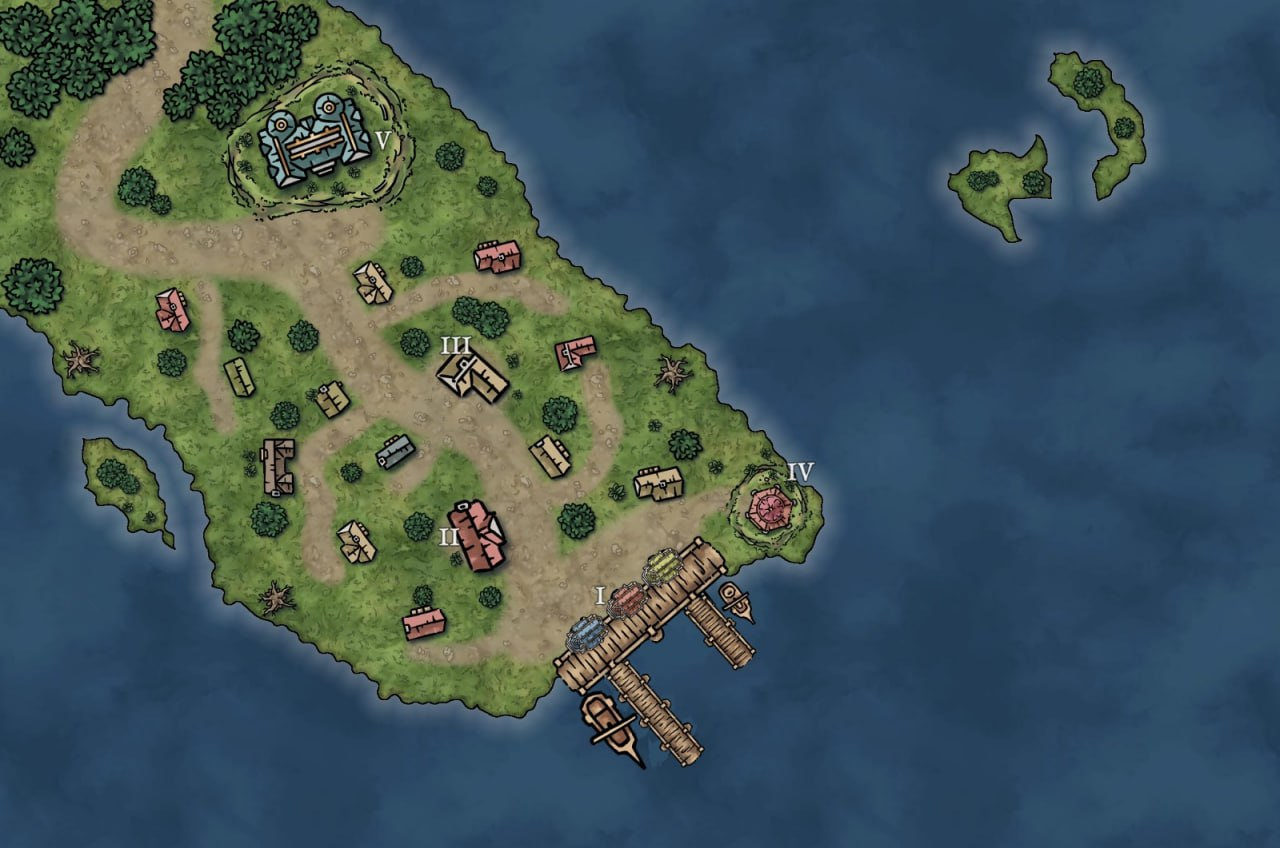
\includegraphics[width=9cm]{./mappe/mappa-middok.png}
\caption{La mappa di Middok}
\label{middok}
\end{figure}


Alla fine di una penisola dove si sviluppa l'abitato di Middok.
Il capitano Vitrovis offre vitto, alloggio e un passaggio in cambio di qualche giorno di lavoro sulla loro nave; il capitano sembra un uomo virtuoso, portano cibo e provviste alla persone del villaggio, con lo scopo di aiutare più che di guadagnare.
Ci si imbatte in tre bancarelle:
\begin{itemize}
  \item Giovane partenopeo mezzorco che vende pesce, il pesce normale è di qualità, quello "raro" probabilmente una truffa
  \item Ragazzo gentile armaiolo, aiuta il padre con la bottega, ci informa sull'affidabilità del vicino mezzorco e ci consiglia di andare dal borgomastro se cerchiamo qualche lavoro
  \item Ragazza halfling (Tamara) che vende strumenti per barca: bussole, quadranti, ecc.
\end{itemize}
Vitrovis litiga con un ragazzino che vuole salire con lui (10-14 anni), il ragazzino scappa tra la folla dopo che Felix lo ha strattonato. Il ragazzino è il figlio del borgomastro.

\subsection{Il borgomastro}
Verso la casa del borgomastro si vede che essa è molto più sfarzosa delle altre; un passante sostiene che non se la passino male, ma che il paese sia sceso di importanza rispetto a un tempo, quando era luogo di partenza e centro della vita dei mari. Il passante riporta che il borgomastro si occupa soprattutto della sua villa e dei nuovi avventurieri, come un normale borgomastro non troppo virtuoso né troppo prepotente.

Il borgomastro Vlaumack ci accoglie, parla della minaccia di temibili pirati avvistati lungo le coste; offre nave e aiuti per andare a respingerli. Il borgomastro risulta sospetto: offre una barca che pare più un relitto, sembra interessato a proteggere le sue ricchezze più che la sua popolazione, elogia gli avventurieri per convincerli a partire, è amico del mezzorco.
Puppies entra in bagno e ruba una saponetta (che è nuova e non rovinata), la domestica ripulisce subito il bagno dopo l'utilizzo.
Il borgomastro offre 15 monete d'oro a test in cambio dei tre pirati che si presume si aggirino in quelle acque (hanno taglie da 20 dobloni ognuno); Stone ha trattato per avere anche il sestante.

\subsection{La locanda}
La locanda è grande, con l'insegna storta; un po' di gente pranza ma non tanta. La vecchietta cordiale è madre del proprietario della locanda e amica di Vitrovis, non è troppo preoccupata per i pirati e indica Zonoi, la vecchia guardiana del faro, che potrebbe avere maggiori informazioni. Zonoi non ha visto pirati se non da bambina, ritiene che il borgomasto abbia ragione a temerli, ma non li ha effettivamente visti nelle vicinanze. Felix fa critico per riparare l'insegna della locanda che era storta, in cambio l'oste offre cena e letto per una notte (Stone dà 2 reals per compassione).

Viene pagato il pranzo per 2 reals; parlando con il proprietario della barca lo aggiorniamo su chi abbiamo incontrato. Gli avventurieri partiti con la nave del borgomastro sono stati depredati e ne è tornato solitamente uno per party.

A pranzo Felix sembra turbato, ansima con il battito accelerato e parla da solo ripetendo ``stai zitto"; Victor comincia a suonare armonica e ukulele per calmare la situazione, ma la gente si ammucchia e Felix si agita ed esce. Victor guadagna due monete per lo spettacolo ed esce per inseguire Felix, che è a pancia in giù steso per terra che dorme. Felix e Victor rientrano, Victor viene acclamato dalla folla.

\subsection{Il faro} Sulla via verso il faro Victor si sgancia dal gruppo e chiede al capitano Vitrovis se sia vera la questione dei pirati, egli riferisce di averli visti. La guardiana del faro vive lì da molti anni con un uccellino, impiegano molto tempo a salire le scale con la vecchietta. Parla di un'isola ``della Luna nascente", a una settimana di navigazione a Est del faro, a Nord - Est altro isolotto e a Nord - Ovest isola molto più abitata ma molto lontana (una decina di giorni di distanza). Zonoi ci regala una bussola. Grande partenza: Zonoi da piccola voleva fare la guardiana del faro da piccola, un tempo Middok era un luogo di grandi partenze. Tamara viene dal mare e si è fermata qua, l'armaiolo è venuto dalla terra. Stone chiede di essere successore del guardiano del faro, Zonoi spera che ci andrà qualcuno di bravo al suo posto.

\subsection{La notte alla Locanda}
Ritorniamo al porto e saliamo sulla barca per controllarla. È un po' più grande di una barca a vela, ha un piano di sotto ed è tutta un po' rovinata, ci sono due cannoni con palle e polvere da sparo; tutto è un po' rovinato; c'è qualche materasso e buchi tappati con assi di legno.

Chiediamo consiglio a Vitruivis, che sta parlando con Carlos (il proprietario della locanda); Vitruvis non è convinto ma dice che possiamo andare se abbiamo bisogno di soldi. Carlos si intromette e dice che i pirati sono temibili e che sembra che la situazione sia complessa, il borgomastro sembra avere molta paura (avendo più da rischiare).

\subsection{Il viaggio}
Il viaggio di mezza giornata, tre giorni di provviste ma dobbiamo restituire il sestante, verso Sud - Est.
\end{document}